\chapter{अभिक्रिया क्रियाविधियाँ: मूल चरण और सन्निकटन}\label{ch:b1:elementary-steps}

कार इंजनों और तड़ित में बनने वाली नाइट्रोजन मोनॉक्साइड हवा की ऑक्सीजन से
संयोग करती है: \ce{2NO + O2 -> 2NO2}। प्रयोगशाला में मापने पर इस अभिक्रिया की
दर $[\ce{NO}]^2[\ce{O2}]$ के समानुपाती मिलती है --- और गैस को गर्म करने पर
अभिक्रिया \emph{धीमी} हो जाती है। तीन अणुओं की एक अकेली टक्कर पहले तथ्य की
व्याख्या कर सकती थी, दूसरे की कभी नहीं: ताप के साथ हर टक्कर अधिक
ऊर्जावान होती जाती है। व्याख्या यह है कि अभिक्रिया एक घटना नहीं, बल्कि
सरलतर घटनाओं का एक क्रम है, उसकी क्रियाविधि। यह अध्याय इन \omterm{def:b1:elementary-steps:elementary-step}{मूल चरणों} को,
उस \omterm{def:b1:elementary-steps:energy-profile}{ऊर्जा प्रोफ़ाइल} को जिसके अनुदिश वे चलते हैं, और उन सन्निकटनों को परिभाषित करता है
जो किसी क्रियाविधि को \omterm{def:b1:rate-laws:order}{दर नियम} में बदलते हैं; अंत में उत्प्रेरण आता है, एक
सरल मार्ग खोलने की कला।

\begin{recall}
पुस्तक 1 (कक्षा 12) ने \omterm{def:b1:elementary-steps:elementary-step}{अभिक्रिया क्रियाविधि} को वक्र तीरों से बनाए गए चरणों के
क्रम के रूप में बताया था, जिसमें मध्यवर्ती बनते और खपते हैं, और
\omterm{def:b1:elementary-steps:catalyst}{उत्प्रेरक} को ऐसी स्पीशीज़ के रूप में जो बिना खपे अभिक्रिया को तेज़ करती है।
\omterm{def:b1:rate-laws:order}{दर नियम}, कोटियाँ और \omterm{thm:b1:rate-laws:arrhenius}{आरेनियस नियम}
\cref{ch:b1:rate-laws} में परिभाषित किए गए।
\end{recall}

\section{मूल चरण}

\begin{definition}[मूल चरण, आण्विकता, क्रियाविधि]\label{def:b1:elementary-steps:elementary-step}
\emph{मूल चरण}\index{मूल चरण} ऐसी अभिक्रिया है जो
एक ही आण्विक घटना में, ठीक वैसे ही जैसे लिखी गई है, बिना किसी
मध्यवर्ती के होती है। इसकी \emph{आण्विकता}\index{आण्विकता} उस घटना में
अभिक्रिया करने वाले कणों की संख्या है: 1 (एकाणुक, कोई विघटन या
पुनर्व्यवस्थापन), 2 (द्विअणुक, एक टक्कर), विरले ही 3। \emph{अभिक्रिया
क्रियाविधि}\index{अभिक्रिया क्रियाविधि} मूल चरणों का वह समुच्चय है जिनका
योग समग्र अभिक्रिया है। जो स्पीशीज़ किसी चरण में बनती है और बाद के किसी चरण में
खपती है, और समग्र समीकरण में नहीं दिखती, वह \emph{अभिक्रिया
मध्यवर्ती}\index{अभिक्रिया मध्यवर्ती} है।
\end{definition}

\begin{proposition}[मूल चरण का दर नियम]\label{prop:b1:elementary-steps:elementary-law}
\omterm{def:b1:elementary-steps:elementary-step}{मूल चरण} की कोटि होती है, और उसकी \omterm{def:b1:rate-laws:order}{आंशिक कोटियाँ} उसके
रससमीकरणमितीय गुणांकों के बराबर होती हैं: $\mathrm{A} \to \dots$ की दर $v = k[\mathrm{A}]$;
$\mathrm{A} + \mathrm{B} \to \dots$ की $v = k[\mathrm{A}][\mathrm{B}]$;
$2\,\mathrm{A} \to \dots$ की $v = k[\mathrm{A}]^2$। विलोम असत्य है:
जिस अभिक्रिया की कोटियाँ उसके गुणांकों के बराबर हों, उसका \omterm{def:b1:elementary-steps:elementary-step}{मूल चरण} होना आवश्यक नहीं।
\end{proposition}

\begin{proof}[तर्क]
द्विअणुक चरण तब होता है जब कोई \ce{A} किसी \ce{B} से मिलता है; प्रति इकाई आयतन
और समय ऐसी भेंटों की संख्या प्रति इकाई आयतन \ce{A} की संख्या
और \ce{B} की संख्या के समानुपाती है, अतः
$[\ce{A}][\ce{B}]$ के। एकाणुक चरण हर अणु के साथ प्रति इकाई समय एक
निश्चित प्रायिकता से होता है, अतः उसकी दर $[\ce{A}]$ के समानुपाती है।
\end{proof}

\begin{remark}[आण्विकता शायद ही दो से अधिक क्यों होती है]\label{rem:b1:elementary-steps:termolecular}
तीन कणों का एक ही क्षण में, हर एक की सही ऊर्जा
और अभिविन्यास के साथ, मिलना एक दुर्लभ घटना है; \omterm{def:b1:rate-laws:order}{समग्र कोटि} 3 की अभिक्रिया लगभग
सदा दो क्रमिक द्विअणुक चरणों का परिणाम होती है, जैसा
सप्ताहांत समस्या में है।
\end{remark}

\section{ऊर्जा प्रोफ़ाइल}

\begin{definition}[अभिक्रिया निर्देशांक, ऊर्जा प्रोफ़ाइल, संक्रमण अवस्था]\label{def:b1:elementary-steps:energy-profile}
किसी \omterm{def:b1:elementary-steps:elementary-step}{मूल चरण} के दौरान परमाणु अभिकारकों की व्यवस्था से
उत्पादों की व्यवस्था की ओर जाते हैं; इस प्रगति को मापने वाला चर
(कोई आबंध लंबाई जो बढ़ती है, कोई दूसरी जो घटती है) \emph{अभिक्रिया
निर्देशांक}\index{अभिक्रिया निर्देशांक} है। उसके अनुदिश निकाय की स्थितिज ऊर्जा
का आलेख \emph{ऊर्जा प्रोफ़ाइल}\index{ऊर्जा प्रोफ़ाइल} है।
इसका उच्चिष्ठ \emph{संक्रमण अवस्था}\index{संक्रमण अवस्था} है,
परमाणुओं की ऐसी व्यवस्था जिसमें आबंध आधे बने और
आधे टूटे होते हैं, जो एक आण्विक कंपन से अधिक नहीं टिकती और जिसे
पृथक नहीं किया जा सकता। अभिकारकों के ऊपर इस उच्चिष्ठ की ऊँचाई चरण का
ऊर्जा अवरोध है।
\end{definition}

\begin{omfigure}
\begin{tikzpicture}
\begin{axis}[omprofile, name=a,
  width=0.48\linewidth, height=5.4cm, xmin=0, xmax=10, ymin=-68, ymax=95,
  xlabel={अभिक्रिया निर्देशांक}, ylabel={ऊर्जा}]
\addplot[omDef, very thick] table[x=x, y=E] {figdata/out/bachelor-1-energy-profiles-one-step.dat};
\draw[dashed, black!40] (axis cs:0,0) -- (axis cs:10,0);
\draw[<->, omThm] (axis cs:5,0) -- (axis cs:5,79);
\node[omThm, anchor=west, font=\small] at (axis cs:5.1,30) {अवरोध};
\draw[<->, omProp] (axis cs:9.9,0) -- (axis cs:9.9,-40);
\node[omProp, anchor=east, font=\small] at (axis cs:9.8,-14) {$\Delta E$};
\node[anchor=south, font=\small] at (axis cs:5,81) {संक्रमण अवस्था};
\node[anchor=north west, font=\small] at (axis cs:0.15,-3) {अभिकारक};
\node[anchor=north, font=\small] at (axis cs:8.6,-42) {उत्पाद};
\end{axis}
\begin{axis}[omprofile, at={(a.east)}, anchor=west, xshift=1.2cm,
  width=0.48\linewidth, height=5.4cm, xmin=0, xmax=10, ymin=-64, ymax=95,
  xlabel={अभिक्रिया निर्देशांक}, ylabel={ऊर्जा}]
\addplot[omDef, very thick] table[x=x, y=E] {figdata/out/bachelor-1-energy-profiles-two-step.dat};
\node[anchor=south, font=\small] at (axis cs:3,71) {सं॰अ॰ 1};
\node[anchor=south, font=\small] at (axis cs:7,56) {सं॰अ॰ 2};
\node[anchor=north, font=\small, align=center] at (axis cs:5,27) {मध्य-\\वर्ती};
\node[anchor=north west, font=\small] at (axis cs:0.15,-3) {अभिकारक};
\node[anchor=north east, font=\small] at (axis cs:10,-43) {उत्पाद};
\end{axis}
\end{tikzpicture}

{\small बाएँ: एक \omterm{def:b1:elementary-steps:elementary-step}{मूल चरण} की प्रोफ़ाइल, उसके अवरोध और
अभिक्रिया के ऊर्जा-परिवर्तन के साथ। दाएँ: दो चरणों वाली क्रियाविधि; मध्यवर्ती
दो \omterm{def:b1:elementary-steps:energy-profile}{संक्रमण अवस्थाओं} (सं॰अ॰) के बीच एक गर्त में बैठता है। ऊर्जाएँ
उदाहरणार्थ हैं।}
\end{omfigure}

\begin{proposition}[अवरोध और आरेनियस नियम]\label{prop:b1:elementary-steps:barrier}
किसी \omterm{def:b1:elementary-steps:elementary-step}{मूल चरण} की \omterm{def:b1:rate-laws:activation-energy}{सक्रियण ऊर्जा} उसके अवरोध के निकट होती है:
केवल वे टक्करें \omterm{def:b1:elementary-steps:energy-profile}{संक्रमण अवस्था} तक पहुँचती हैं जो कम-से-कम उतनी ऊर्जा लाती हैं।
किसी चरण की अग्र और प्रतीप दिशाओं के लिए $E_{a,+} -
E_{a,-} = \Delta E$, जो चरण की अभिक्रिया-ऊर्जा है।
\end{proposition}

\begin{proof}[तर्क]
प्रतीप चरण उसी अवरोध पर दूसरी ओर से चढ़ता है: उत्पादों से मापी गई उसकी
ऊँचाई अग्र ऊँचाई से $-\Delta E$ अधिक है।
\end{proof}

\begin{proposition}[हैमंड अभिगृहीत]\label{prop:b1:elementary-steps:hammond}
किसी \omterm{def:b1:elementary-steps:elementary-step}{मूल चरण} की \omterm{def:b1:elementary-steps:energy-profile}{संक्रमण अवस्था} संरचना और ऊर्जा में उस स्पीशीज़ से मिलती-जुलती है
जिसके वह ऊर्जा में अधिक निकट है: प्रबल रूप से चढ़ाई वाले (ऊष्माशोषी) चरण के लिए
उत्पादों से, प्रबल रूप से ढलान वाले (ऊष्माक्षेपी) चरण के लिए अभिकारकों से।
फलतः, उच्च-ऊर्जा मध्यवर्ती बनाने वाले चरण के लिए, जो कुछ भी
मध्यवर्ती को स्थायित्व देता है वह उस तक ले जाने वाले अवरोध को भी
घटाता है।
\end{proposition}
\admitted

\section{दर-निर्धारक चरण और पूर्व-साम्य}

\begin{definition}[दर-निर्धारक चरण]\label{def:b1:elementary-steps:rds}
चरणों के किसी क्रम में \emph{दर-निर्धारक
चरण}\index{दर-निर्धारक चरण} वह चरण है जो बाक़ी सभी चरणों से बहुत धीमा हो;
समग्र दर उसकी दर के बराबर होती है, और तेज़ चरण उसके अनुसार
ढल जाते हैं, जैसे किसी सड़क की गाड़ियाँ उसके सबसे धीमे बिंदु के पीछे चलती हैं।
\end{definition}

\begin{definition}[पूर्व-साम्य सन्निकटन]\label{def:b1:elementary-steps:pre-equilibrium}
\emph{पूर्व-साम्य सन्निकटन}\index{पूर्व-साम्य सन्निकटन} में
\omterm{def:b1:elementary-steps:rds}{दर-निर्धारक चरण} से पहले आने वाले तीव्र उत्क्रमणीय चरण को
पूरे समय साम्य में माना जाता है: उसकी स्पीशीज़ की सांद्रताएँ
उसके साम्य स्थिरांक $K_1 = k_1/k_{-1}$ का पालन करती हैं।
\end{definition}

\begin{proposition}[पूर्व-साम्य से दर नियम]\label{prop:b1:elementary-steps:pre-equilibrium-law}
क्रियाविधि
\[
  \mathrm{A} + \mathrm{B} \underset{k_{-1}}{\overset{k_1}{\rightleftharpoons}} \mathrm{I}
  \ \text{(तीव्र)}, \qquad
  \mathrm{I} + \mathrm{C} \xrightarrow{\ k_2\ } \mathrm{P} \ \text{(मंद)},
\]
के लिए दर $v = k_2K_1[\mathrm{A}][\mathrm{B}][\mathrm{C}]$ है, \omterm{def:b1:rate-laws:order}{समग्र
कोटि} 3, आभासी स्थिरांक $k = k_1k_2/k_{-1}$ के साथ।
\end{proposition}

\begin{proof}
दर मंद चरण की दर है, $v = k_2[\mathrm{I}][\mathrm{C}]$।
पहला चरण साम्य में रहता है: $k_1[\mathrm{A}][\mathrm{B}] =
k_{-1}[\mathrm{I}]$, इसलिए $[\mathrm{I}] = K_1[\mathrm{A}][\mathrm{B}]$।
प्रतिस्थापन से परिणाम मिलता है।
\end{proof}

\section{स्थायी-अवस्था सन्निकटन}

\begin{theorem}[क्रमागत प्रथम कोटि अभिक्रियाएँ]\label{thm:b1:elementary-steps:consecutive}
$\mathrm{A} \xrightarrow{k_1} \mathrm{B} \xrightarrow{k_2} \mathrm{C}$ के लिए,
जहाँ दोनों चरण कोटि 1 के हैं, $[\mathrm{A}] = a_0$ और $[\mathrm{B}] =
[\mathrm{C}] = 0$, $t = 0$ पर, और $k_1 \ne k_2$:
\[
  [\mathrm{A}] = a_0\eu^{-k_1t}, \qquad
  [\mathrm{B}] = \frac{a_0k_1}{k_2 - k_1}\big(\eu^{-k_1t} - \eu^{-k_2t}\big),
  \qquad [\mathrm{C}] = a_0 - [\mathrm{A}] - [\mathrm{B}] .
\]
मध्यवर्ती एक उच्चिष्ठ से गुज़रता है, $t_{\max} = \dfrac{\ln(k_2/k_1)}
{k_2 - k_1}$ पर।
\end{theorem}

\begin{proof}
$\dd[\mathrm{A}]/\dd t = -k_1[\mathrm{A}]$ से $[\mathrm{A}]$ मिलता है। तब
$\dd[\mathrm{B}]/\dd t + k_2[\mathrm{B}] = k_1a_0\eu^{-k_1t}$, एक प्रथम कोटि का
रैखिक समीकरण है: $\eu^{k_2t}$ से गुणा करने पर $\frac{\dd}{\dd t}
\big([\mathrm{B}]\eu^{k_2t}\big) = k_1a_0\eu^{(k_2-k_1)t}$, जिसका
0 से समाकल, जहाँ $[\mathrm{B}] = 0$, $[\mathrm{B}]\eu^{k_2t} =
\frac{k_1a_0}{k_2-k_1}(\eu^{(k_2-k_1)t} - 1)$ है। द्रव्य-संरक्षण से
$[\mathrm{C}]$ मिलता है। $[\mathrm{B}]$ का अवकलज तब शून्य होता है जब $k_1\eu^{-k_1t}
= k_2\eu^{-k_2t}$, अर्थात् $t_{\max}$ पर।
\end{proof}

\begin{definition}[स्थायी-अवस्था सन्निकटन]\label{def:b1:elementary-steps:qssa}
\emph{स्थायी-अवस्था सन्निकटन}\index{स्थायी-अवस्था सन्निकटन}
(या अर्ध-स्थायी अवस्था) में, किसी अत्यधिक
क्रियाशील मध्यवर्ती की सांद्रता, जो बनने से कहीं तेज़ी से खपता है, एक छोटी
प्रेरण-अवधि के बाद स्थिर और छोटी मानी जाती है: उसकी
\omterm{def:b1:rate-laws:rate}{निर्माण दर} उसकी खपत दर के बराबर होती है,
$\dd[\mathrm{I}]/\dd t \approx 0$।
\end{definition}

\begin{proposition}[स्थायी अवस्था कब मान्य है]\label{prop:b1:elementary-steps:qssa-justified}
$\mathrm{A} \to \mathrm{B} \to \mathrm{C}$ के लिए, जहाँ $k_2 \gg k_1$: लगभग
$1/k_2$ की कोटि के समय के बाद $[\mathrm{B}] \approx k_1[\mathrm{A}]/k_2$ (जो
$\dd[\mathrm{B}]/\dd t = 0$ से मिलता है), $[\mathrm{B}]$ छोटा बना रहता है, और
उत्पाद $\dd[\mathrm{C}]/\dd t \approx k_1[\mathrm{A}]$ की दर से बनता है:
पहला चरण दर-निर्धारक है।
\end{proposition}

\begin{proof}
$k_2 \gg k_1$ और $t \gg 1/k_2$ के लिए $\eu^{-k_2t}$,
$\eu^{-k_1t}$ की तुलना में नगण्य है और $k_2 - k_1 \approx k_2$, इसलिए $[\mathrm{B}] \approx (a_0k_1/k_2)
\eu^{-k_1t} = k_1[\mathrm{A}]/k_2 \ll [\mathrm{A}]$। तब
$\dd[\mathrm{C}]/\dd t = k_2[\mathrm{B}] \approx k_1[\mathrm{A}]$।
\end{proof}

\begin{omfigure}
\begin{tikzpicture}
\begin{axis}[name=s,
  width=0.48\linewidth, height=5.2cm, xmin=0, xmax=6, ymin=0, ymax=1.05,
  axis x line=bottom, axis y line=left,
  xlabel={$k_1t$}, ylabel={सांद्रता$/a_0$},
  title={$k_2 = 0.5\,k_1$}, title style={font=\small},
  tick label style={font=\small}, label style={font=\small}]
\addplot[omDef, thick] table[x=t, y=a] {figdata/out/bachelor-1-consecutive-reactions-slow.dat};
\addplot[omThm, thick] table[x=t, y=b] {figdata/out/bachelor-1-consecutive-reactions-slow.dat};
\addplot[omMeth, thick] table[x=t, y=c] {figdata/out/bachelor-1-consecutive-reactions-slow.dat};
\node[omDef, font=\small, anchor=west] at (axis cs:0.4,0.75) {A};
\node[omThm, font=\small, anchor=south] at (axis cs:1.39,0.51) {B};
\node[omMeth, font=\small, anchor=west] at (axis cs:4.5,0.75) {C};
\end{axis}
\begin{axis}[at={(s.east)}, anchor=west, xshift=1.2cm,
  width=0.48\linewidth, height=5.2cm, xmin=0, xmax=6, ymin=0, ymax=1.05,
  axis x line=bottom, axis y line=left,
  xlabel={$k_1t$}, ylabel={सांद्रता$/a_0$},
  title={$k_2 = 20\,k_1$}, title style={font=\small},
  tick label style={font=\small}, label style={font=\small}]
\addplot[omDef, thick] table[x=t, y=a] {figdata/out/bachelor-1-consecutive-reactions-fast.dat};
\addplot[omThm, thick] table[x=t, y=b] {figdata/out/bachelor-1-consecutive-reactions-fast.dat};
\addplot[omMeth, thick] table[x=t, y=c] {figdata/out/bachelor-1-consecutive-reactions-fast.dat};
\addplot[black, dashed] table[x=t, y=bss] {figdata/out/bachelor-1-consecutive-reactions-fast.dat};
\node[omDef, font=\small, anchor=west] at (axis cs:1.4,0.32) {A};
\node[omThm, font=\small, anchor=south west] at (axis cs:2,0.22) {B (स्थायी अवस्था: डैश)};
\node[omMeth, font=\small, anchor=west] at (axis cs:4.5,0.85) {C};
\end{axis}
\end{tikzpicture}

{\small क्रमागत अभिक्रियाएँ $\mathrm{A} \to \mathrm{B} \to \mathrm{C}$।
बाएँ: मध्यवर्ती संचित होता है और $k_1t = 1.39$ पर शिखर पर पहुँचता है। दाएँ:
जब वह बनने से बीस गुना तेज़ी से खपता है, तो वह छोटा रहता है और
एक संक्षिप्त प्रेरण के बाद स्थायी-अवस्था मान $k_1[\mathrm{A}]/k_2$ (डैश) का
अनुसरण करता है।}
\end{omfigure}

\begin{method}[क्रियाविधि से दर नियम]\label{met:b1:elementary-steps:rate-law}
किसी क्रियाविधि का \omterm{def:b1:rate-laws:order}{दर नियम} व्युत्पन्न करने के लिए:
\begin{enumerate}
  \item हर \omterm{def:b1:elementary-steps:elementary-step}{मूल चरण} की दर लिखिए (\cref{prop:b1:elementary-steps:elementary-law});
  \item समग्र दर को किसी उत्पाद की \omterm{def:b1:rate-laws:rate}{निर्माण दर} के रूप में व्यक्त कीजिए
        (उसके गुणांक से भाग देकर);
  \item हर मध्यवर्ती का निरसन \omterm{def:b1:elementary-steps:qssa}{स्थायी-अवस्था सन्निकटन} से कीजिए
        ($\dd[\mathrm{I}]/\dd t = 0$, एक बीजीय समीकरण), या, यदि कोई तीव्र
        साम्य किसी मंद चरण से पहले आता हो, तो उसके स्थिरांक से;
  \item उन सीमाओं में सरल कीजिए जहाँ कोई एक पद प्रधान हो, और
        प्रायोगिक नियम से तुलना कीजिए।
\end{enumerate}
\end{method}

\begin{example}[एक अम्ल-उत्प्रेरित अभिक्रिया]\label{ex:b1:elementary-steps:acid}
$\mathrm{S} + \ce{H3O+} \rightleftharpoons \mathrm{SH}^+ + \ce{H2O}$ (तीव्र,
स्थिरांक $K_1$) के बाद $\mathrm{SH}^+ + \ce{H2O} \to \mathrm{P} + \ce{H3O+}$ (मंद,
$k_2$) के लिए दर $v = k_2[\mathrm{SH}^+] = k_2K_1[\mathrm{S}][\ce{H3O+}]$ है:
क्रियाधार में और अम्ल में प्रथम कोटि, यद्यपि अम्ल खपता नहीं।
\end{example}

\section{उत्प्रेरण और वरणात्मकता का नियंत्रण}

\begin{definition}[उत्प्रेरक, समांगी और विषमांगी उत्प्रेरण]\label{def:b1:elementary-steps:catalyst}
\emph{उत्प्रेरक}\index{उत्प्रेरक} ऐसी स्पीशीज़ है जो किसी अभिक्रिया की दर बढ़ाती है
पर उसके समग्र समीकरण में नहीं आती: क्रियाविधि के किसी एक चरण में
खपकर वह बाद के किसी चरण में पुनः बन जाती है।
\emph{समांगी उत्प्रेरण}\index{समांगी उत्प्रेरण} में उत्प्रेरक
अभिकारकों की ही \omterm{def:b1:extent-q-and-k:system}{प्रावस्था} में होता है (घुले हुए अम्ल, धातु संकुल,
एंज़ाइम); \emph{विषमांगी उत्प्रेरण}\index{विषमांगी उत्प्रेरण} में
वह एक अलग \omterm{def:b1:extent-q-and-k:system}{प्रावस्था} होता है, प्रायः एक ठोस जिसकी सतह पर
अभिक्रिया होती है (प्लैटिनम, आयरन, ज़िओलाइट)।
\end{definition}

\begin{proposition}[उत्प्रेरक क्या बदलता है]\label{prop:b1:elementary-steps:catalysis}
\omterm{def:b1:elementary-steps:catalyst}{उत्प्रेरक} कम अवरोध वाली एक नई क्रियाविधि प्रदान करता है। वह
अग्र और प्रतीप अभिक्रियाओं को एक ही अनुपात में तेज़ करता है, और इसलिए
साम्य स्थिरांक, अंतिम अवस्था और अभिक्रिया-ऊर्जा को
अपरिवर्तित छोड़ता है।
\end{proposition}

\begin{proof}
साम्य पर किसी \omterm{def:b1:elementary-steps:elementary-step}{मूल चरण} के लिए अग्र और प्रतीप दरें
बराबर होती हैं: $k_+[\text{अभिकारक}] = k_-[\text{उत्पाद}]$, इसलिए $K = k_+/k_-$।
साम्य पर किसी भी क्रियाविधि के लिए हर चरण साम्य में होता है (अन्यथा
कोई स्पीशीज़ बदलती रहती), और $K$ चरणों के अनुपातों $k_+/k_-$ का
गुणनफल है। उत्प्रेरित मार्ग उसी अंतिम अवस्था तक, उसी स्थिरांक के साथ,
पहुँचता है: वह $k_+$ को जिस गुणक से भी गुणा करे, $k_-$ को
भी उसी गुणक से गुणा करता है।
\end{proof}

\begin{omfigure}
\begin{tikzpicture}
\begin{axis}[omprofile,
  width=0.62\linewidth, height=5.6cm, xmin=0, xmax=10, ymin=-45, ymax=115,
  xlabel={अभिक्रिया निर्देशांक}, ylabel={ऊर्जा}]
\addplot[black!60, very thick] table[x=x, y=E] {figdata/out/bachelor-1-energy-profiles-uncatalysed.dat};
\addplot[omMeth, very thick] table[x=x, y=E] {figdata/out/bachelor-1-energy-profiles-catalysed.dat};
\node[anchor=south, font=\small] at (axis cs:5,101) {उत्प्रेरक के बिना};
\node[omMeth, anchor=north, font=\small] at (axis cs:3.5,-6) {उत्प्रेरक के साथ};
\draw[<->, omProp] (axis cs:10.4,0) -- (axis cs:10.4,-30);
\draw[dashed, black!40] (axis cs:0,0) -- (axis cs:10.6,0);
\node[omProp, anchor=west, font=\small] at (axis cs:10.5,-15) {$\Delta E$ अपरिवर्तित};
\end{axis}
\end{tikzpicture}

{\small \omterm{def:b1:elementary-steps:catalyst}{उत्प्रेरक} कम अवरोधों वाला एक मार्ग खोलता है (हरा), प्रायः
कई चरणों में; आरंभ और अंत, अतः अभिक्रिया-ऊर्जा और
साम्य, वही रहते हैं।}
\end{omfigure}

\begin{omfigure}
\begin{tikzpicture}[font=\small, >={Stealth}]
  \node[draw=omMeth, rounded corners, fill=omMeth!10, minimum width=2.4cm] (c) at (0,1.6) {उत्प्रेरक};
  \node[draw=black!50, rounded corners, fill=black!5, minimum width=2.4cm] (i1) at (2.6,0) {संकुल 1};
  \node[draw=black!50, rounded corners, fill=black!5, minimum width=2.4cm] (i2) at (0,-1.6) {संकुल 2};
  \node[draw=black!50, rounded corners, fill=black!5, minimum width=2.4cm] (i3) at (-2.6,0) {संकुल 3};
  \draw[->, thick] (c) to[bend left=20] node[above right] {+ A} (i1);
  \draw[->, thick] (i1) to[bend left=20] node[below right] {+ B} (i2);
  \draw[->, thick] (i2) to[bend left=20] node[below left] {} (i3);
  \draw[->, thick] (i3) to[bend left=20] node[above left] {$-$ P} (c);
\end{tikzpicture}

{\small एक \omterm{def:b1:elementary-steps:catalyst}{उत्प्रेरक} चक्र: \omterm{def:b1:elementary-steps:catalyst}{उत्प्रेरक} बारी-बारी से अभिकारकों A और B को बाँधता है,
उत्पाद P मुक्त होता है, और \omterm{def:b1:elementary-steps:catalyst}{उत्प्रेरक} पुनः बनकर फिर से
आरंभ करता है। धातु संकुलों के \omterm{def:b1:elementary-steps:catalyst}{उत्प्रेरक} चक्रों का अध्ययन द्वितीय वर्ष के
खंड में होता है।}
\end{omfigure}

\begin{omfigure}
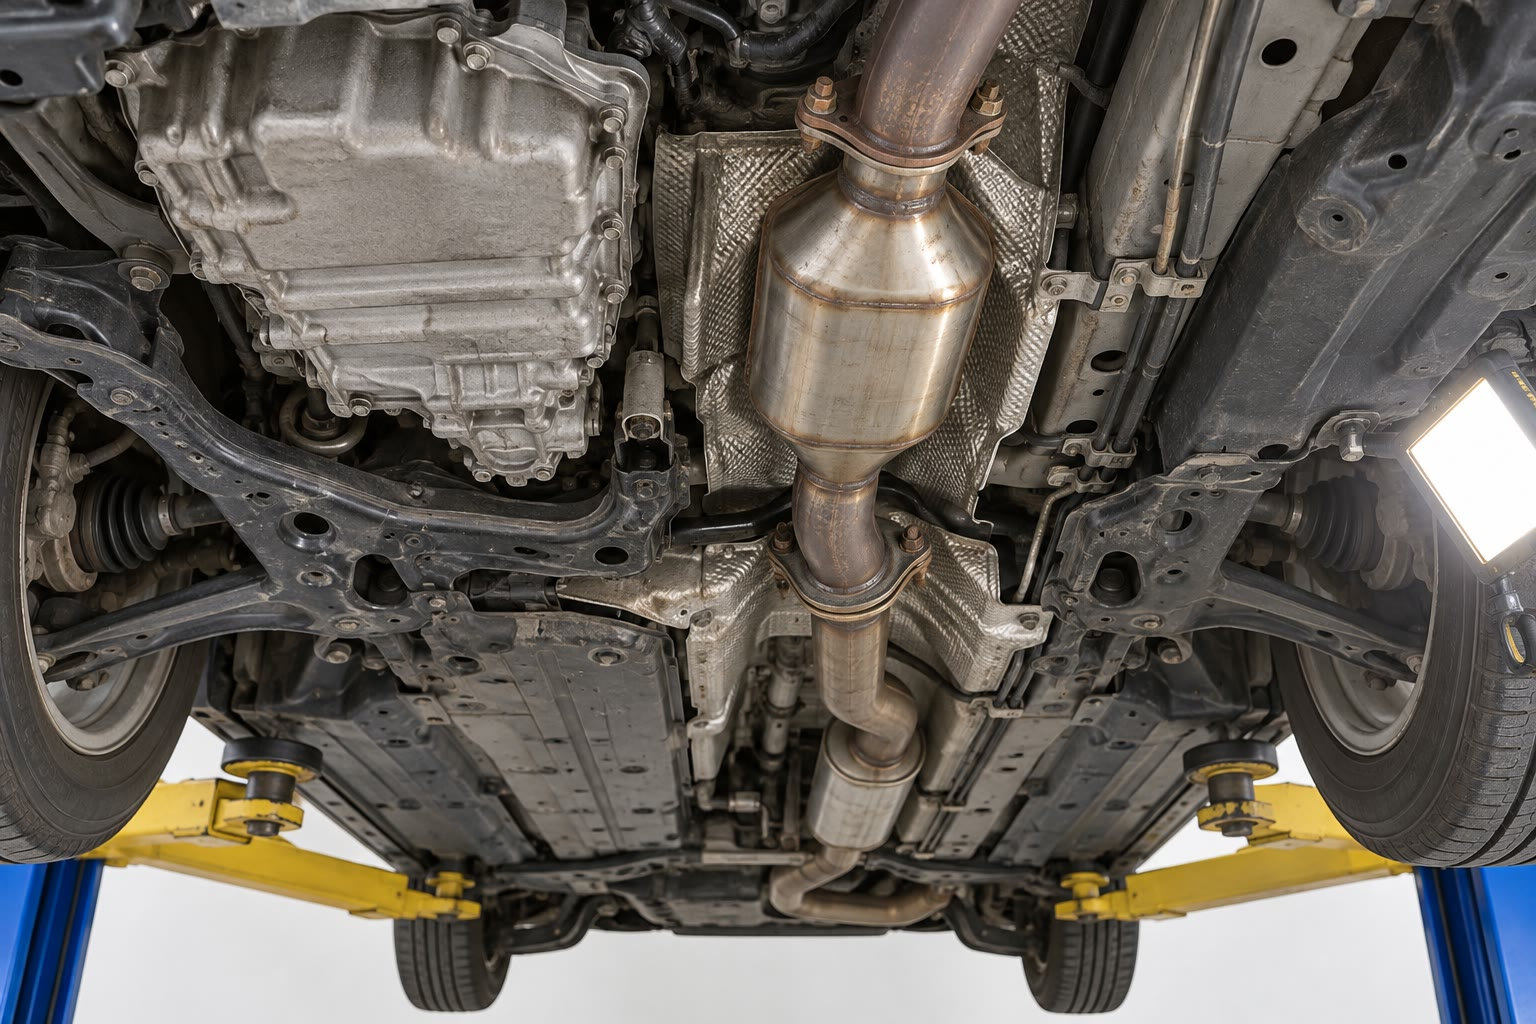
\includegraphics[width=0.5\linewidth]{images/book2/ai/b1-09-catalytic-converter.jpg}

{\small कार का निचला भाग: निकास-नली में लगा डिब्बा एक
\omterm{def:b1:elementary-steps:catalyst}{उत्प्रेरक} परिवर्तक है, एक विषमांगी \omterm{def:b1:elementary-steps:catalyst}{उत्प्रेरक} जिसकी धात्विक सतह पर
निकास गैसें अभिक्रिया करती हैं।}
\end{omfigure}

\begin{definition}[गतिक और ऊष्मागतिक नियंत्रण]\label{def:b1:elementary-steps:control}
जब कोई अभिकारक प्रतिस्पर्धी मार्गों से दो उत्पाद दे सकता है, तो अभिक्रिया
\emph{गतिक नियंत्रण}\index{गतिक नियंत्रण} में होती है यदि उत्पादों के
अनुपात निर्माण की दरों से तय हों (कम अवरोध वाला
उत्पाद प्रधान होता है), और \emph{ऊष्मागतिक
नियंत्रण}\index{ऊष्मागतिक नियंत्रण} में यदि मार्ग उत्क्रमणीय हों और
निकाय साम्य तक पहुँच जाए (अधिक स्थायी उत्पाद प्रधान होता है)।
\end{definition}

\begin{example}[उत्पाद का चुनाव]\label{ex:b1:elementary-steps:control}
कोई अभिकारक \qty{50}{kJ/mol} के अवरोध पर B देता है ($\Delta E =
\qty{-10}{kJ/mol}$) और \qty{70}{kJ/mol} के अवरोध पर C ($\Delta E =
\qty{-40}{kJ/mol}$)। \qty{300}{K} पर और कम समयों में, समान
\omterm{def:b1:rate-laws:activation-energy}{पूर्व-घातांकी गुणकों} के साथ, B, C से $\exp(20000/(8.314 \times 300)) \approx
3000$ गुना तेज़ी से बनता है: \omterm{def:b1:elementary-steps:control}{गतिक नियंत्रण} B देता है। ऊँचे ताप पर
और लंबे समयों में B अपने छोटे प्रतीप अवरोध को पार करके लौट जाता है, C नहीं, और
निकाय C पर समाप्त होता है: \omterm{def:b1:elementary-steps:control}{ऊष्मागतिक नियंत्रण}।
\end{example}

\begin{history}[उत्प्रेरण, 1835]
1835 में स्वीडिश रसायनज्ञ योन्स याकोब बर्ज़ीलियस ने एक ही शब्द के अंतर्गत
दर्जन भर उलझाने वाले प्रेक्षण इकट्ठे किए --- अम्लों द्वारा स्टार्च का शर्करा में बदलना,
धातुओं द्वारा हाइड्रोजन परॉक्साइड का विघटन, प्लैटिनम पर ऐल्कोहॉल का ऑक्सीकरण ---
और वहाँ कार्यरत छिपे बल को ``\omterm{def:b1:elementary-steps:catalyst}{उत्प्रेरक}'' कहा। \omterm{def:b1:elementary-steps:catalyst}{उत्प्रेरक} को ऐसी स्पीशीज़ के रूप में परिभाषित करने के लिए,
जो अभिक्रिया की दर बदलती है पर उसका साम्य नहीं, सदी के अंत की बलगतिकी और
विल्हेल्म ऑस्टवाल्ड की आवश्यकता पड़ी।
\end{history}

\section{अभ्यास}

\begin{exercise}[$\star$]\label{exo:b1:elementary-steps:1}
हर चरण की \omterm{def:b1:elementary-steps:elementary-step}{आण्विकता} बताइए और बताइए कि कौन-से चरण \omterm{def:b1:elementary-steps:elementary-step}{मूल चरण} हो सकते हैं:
(a) $\ce{N2O5 -> NO2 + NO3}$; (b) $\ce{NO + NO3 -> 2NO2}$;
(c) $\ce{2H2 + O2 -> 2H2O}$; (d) $\ce{O + O2 + N2 -> O3 + N2}$।
\end{exercise}

\begin{exercise}[$\star$]\label{exo:b1:elementary-steps:2}
\omterm{def:b1:elementary-steps:elementary-step}{मूल चरणों} $\mathrm{A} + \mathrm{B} \to
\mathrm{C}$, $2\,\mathrm{A} \to \mathrm{B}$ और $\mathrm{A} \to \mathrm{B} +
\mathrm{C}$ के \omterm{def:b1:rate-laws:order}{दर नियम} लिखिए। किसी समग्र अभिक्रिया का \omterm{def:b1:rate-laws:order}{दर नियम} उसके
समीकरण से क्यों नहीं लिखा जा सकता?
\end{exercise}

\begin{exercise}[$\star$]\label{exo:b1:elementary-steps:3}
इस अध्याय में बनी दो-चरणी \omterm{def:b1:elementary-steps:energy-profile}{ऊर्जा प्रोफ़ाइल} पर (मध्यवर्ती
30 पर, \omterm{def:b1:elementary-steps:energy-profile}{संक्रमण अवस्थाएँ} 70 और 55 पर, उत्पाद $-40$ पर, अभिकारकों के ऊपर
\unit{kJ/mol} में), मध्यवर्ती, \omterm{def:b1:elementary-steps:energy-profile}{संक्रमण अवस्थाएँ} और \omterm{def:b1:elementary-steps:rds}{दर-निर्धारक चरण} पहचानिए।
क्या पहला चरण ऊष्माशोषी है या ऊष्माक्षेपी?
\end{exercise}

\begin{exercise}[$\star$]\label{exo:b1:elementary-steps:4}
कोई \omterm{def:b1:elementary-steps:catalyst}{उत्प्रेरक} किसी \omterm{def:b1:elementary-steps:elementary-step}{मूल चरण} के अग्र \omterm{def:b1:rate-laws:order}{दर स्थिरांक} को
$10^4$ से गुणा करता है। वह प्रतीप \omterm{def:b1:rate-laws:order}{दर स्थिरांक} को कितने से गुणा करता है? साम्य
स्थिरांक को? साम्य तक पहुँचने के लिए आवश्यक समय को?
\end{exercise}

\begin{exercise}[$\star\star$]\label{exo:b1:elementary-steps:5}
$\mathrm{A} \to \mathrm{B} \to \mathrm{C}$ के लिए, जहाँ $k_1 =
\qty{0.10}{s^{-1}}$ और $k_2 = \qty{0.30}{s^{-1}}$, $t_{\max}$ और
$\mathrm{B}$ की सबसे बड़ी सांद्रता, $a_0$ की इकाई में, परिकलित कीजिए।
\end{exercise}

\begin{exercise}[$\star\star$]\label{exo:b1:elementary-steps:6}
$\mathrm{A} \underset{k_{-1}}{\overset{k_1}{\rightleftharpoons}}
\mathrm{I} \xrightarrow{k_2} \mathrm{P}$ के लिए, जहाँ सभी चरण कोटि 1 के हैं,
$\mathrm{I}$ पर \omterm{def:b1:elementary-steps:qssa}{स्थायी-अवस्था सन्निकटन} लगाइए और दिखाइए कि $v =
\frac{k_1k_2}{k_{-1} + k_2}[\mathrm{A}]$। स्थितियों $k_2 \gg
k_{-1}$ और $k_2 \ll k_{-1}$ पर विचार कीजिए।
\end{exercise}

\begin{exercise}[$\star\star$]\label{exo:b1:elementary-steps:7}
आयोडाइड आयन हाइड्रोजन परॉक्साइड के विघटन को उत्प्रेरित करते हैं:
\ce{H2O2 + I- -> H2O + IO-} (मंद), फिर \ce{H2O2 + IO- -> H2O + O2 + I-}
(तीव्र)। समग्र समीकरण लिखिए, \omterm{def:b1:elementary-steps:catalyst}{उत्प्रेरक} और
मध्यवर्ती पहचानिए, और \omterm{def:b1:rate-laws:order}{दर नियम} बताइए।
\end{exercise}

\begin{exercise}[$\star\star$]\label{exo:b1:elementary-steps:8}
कोई चरण किसी उदासीन अणु से कार्बधनायन बनाता है, जो प्रबल रूप से चढ़ाई वाला
प्रक्रम है। हैमंड अभिगृहीत की सहायता से समझाइए कि कार्बधनायन को
स्थायित्व देने वाला प्रतिस्थापी चरण को भी तेज़ क्यों करता है।
\end{exercise}

\begin{exercise}[$\star\star$]\label{exo:b1:elementary-steps:9}
\cref{ex:b1:elementary-steps:control} में \qty{300}{K} पर और \qty{600}{K} पर
B और C के निर्माण के \omterm{def:b1:rate-laws:order}{दर स्थिरांकों} का अनुपात परिकलित कीजिए।
टिप्पणी कीजिए।
\end{exercise}

\begin{exercise}[$\star\star\star$]\label{exo:b1:elementary-steps:10}
एक गैस $\mathrm{A}$ किसी भी
अणु $\mathrm{M}$ से टक्कर द्वारा सक्रियित होने के बाद विघटित होती है: $\mathrm{A} + \mathrm{M} \rightleftharpoons
\mathrm{A}^* + \mathrm{M}$ ($k_1$, $k_{-1}$), फिर $\mathrm{A}^* \to
\mathrm{P}$ ($k_2$)। $\mathrm{A}^*$ के लिए \omterm{def:b1:elementary-steps:qssa}{स्थायी-अवस्था सन्निकटन} से
$v$ ज्ञात कीजिए, और दिखाइए कि अभिक्रिया उच्च दाब पर कोटि 1 की
और निम्न दाब पर कोटि 2 की होती है।
\end{exercise}

\begin{exercise}[$\star\star\star$]\label{exo:b1:elementary-steps:11}
\cref{thm:b1:elementary-steps:consecutive} के $[\mathrm{B}](t)$ का सूत्र सिद्ध
कीजिए और विशेष स्थिति $k_1 = k_2 = k$ पर विचार कीजिए, जिसके लिए
$[\mathrm{B}] = a_0kt\,\eu^{-kt}$।
\end{exercise}

\begin{exercise}[$\star\star\star$]\label{exo:b1:elementary-steps:12}
समग्र अभिक्रिया $\mathrm{A} + 2\,\mathrm{B} \to \mathrm{P} +
\mathrm{C}$ का प्रायोगिक \omterm{def:b1:rate-laws:order}{दर नियम} $v =
k[\mathrm{A}][\mathrm{B}]^2/[\mathrm{C}]$ है। तीव्र पूर्व-साम्य वाली एक क्रियाविधि
प्रस्तावित कीजिए जो इसकी व्याख्या करे।
\end{exercise}

\section{समस्या: नाइट्रोजन मोनॉक्साइड ठंड में तेज़ी से ऑक्सीकृत क्यों होती है}

\begin{problem}[{सप्ताहांत समस्या --- नाइट्रोजन मोनॉक्साइड का तृतीय कोटि का
ऑक्सीकरण, द्वितय \ce{N2O2} के माध्यम से पूर्व-साम्य, स्थायी-अवस्था
विवेचन, और ऋणात्मक आभासी \omterm{def:b1:rate-laws:activation-energy}{सक्रियण ऊर्जा}}]
\label{pb:b1:elementary-steps:1}
\ce{2NO(g) + O2(g) -> 2NO2(g)} के लिए \qty{300}{K} पर \omterm{def:b1:rate-laws:initial-rate}{प्रारंभिक दरों} के मापन ये
देते हैं (दरें \unit{mol.L^{-1}.s^{-1}} में):
\begin{center}
\begin{tabular}{cccc}
\hline
प्रयोग & $[\ce{NO}]_0$ (mol/L) & $[\ce{O2}]_0$ (mol/L) & $v_0$ \\
\hline
1 & \num{1.0e-3} & \num{1.0e-3} & \num{1.0e-5} \\
2 & \num{2.0e-3} & \num{1.0e-3} & \num{4.0e-5} \\
3 & \num{1.0e-3} & \num{2.0e-3} & \num{2.0e-5} \\
\hline
\end{tabular}
\end{center}
\qty{400}{K} पर प्राप्त \omterm{def:b1:rate-laws:order}{दर स्थिरांक} \qty{300}{K} वाले से दस गुना
छोटा है। $R = \qty{8.314}{J/(mol.K)}$ लीजिए।
प्रस्तावित क्रियाविधि है
\[
  \ce{2NO <=> N2O2} \ \ (k_1, k_{-1}, \text{तीव्र}), \qquad
  \ce{N2O2 + O2 -> 2NO2} \ \ (k_2, \text{मंद}).
\]

\medskip
\noindent\textbf{भाग I --- प्रेक्षित नियम।}
\begin{enumerate}
  \item \ce{NO} और \ce{O2} के सापेक्ष \omterm{def:b1:rate-laws:order}{आंशिक कोटियाँ} ज्ञात कीजिए।
  \item \omterm{def:b1:rate-laws:order}{दर नियम} लिखिए और \qty{300}{K} पर $k$, उसके मात्रक सहित, परिकलित कीजिए।
  \item क्या अभिक्रिया एक अकेला त्रिअणुक चरण हो सकती है? एक तर्क दीजिए।
  \item दोनों तापों से आभासी \omterm{def:b1:rate-laws:activation-energy}{सक्रियण ऊर्जा} परिकलित कीजिए।
  \item किसी \omterm{def:b1:elementary-steps:elementary-step}{मूल चरण} के लिए ऋणात्मक \omterm{def:b1:rate-laws:activation-energy}{सक्रियण ऊर्जा} असंभव क्यों है?
  \item \ce{NO} और \ce{O2} की \omterm{def:b1:rate-laws:rate}{लोप दरें}
        $v$ के रूप में लिखिए।
\end{enumerate}

\medskip
\noindent\textbf{भाग II --- पूर्व-साम्य।}
\begin{enumerate}[resume]
  \item जाँचिए कि दोनों चरणों का योग समग्र अभिक्रिया है। मध्यवर्ती
        का नाम बताइए।
  \item हर चरण की \omterm{def:b1:elementary-steps:elementary-step}{आण्विकता} बताइए।
  \item मंद चरण की दर लिखिए।
  \item \omterm{def:b1:elementary-steps:pre-equilibrium}{पूर्व-साम्य सन्निकटन} से $[\ce{N2O2}]$ व्यक्त कीजिए।
  \item \omterm{def:b1:rate-laws:order}{दर नियम} निकालिए और प्रयोग से तुलना कीजिए।
  \item प्रेक्षित स्थिरांक को $k_1$, $k_{-1}$ और $k_2$ के रूप में व्यक्त कीजिए।
\end{enumerate}

\medskip
\noindent\textbf{भाग III --- स्थायी अवस्था।}
\begin{enumerate}[resume]
  \item पूरी क्रियाविधि के लिए $\dd[\ce{N2O2}]/\dd t$ लिखिए।
  \item \omterm{def:b1:elementary-steps:qssa}{स्थायी-अवस्था सन्निकटन} लगाइए और $[\ce{N2O2}]$ व्यक्त कीजिए।
  \item \omterm{def:b1:rate-laws:order}{दर नियम} $v = \dfrac{k_1k_2[\ce{NO}]^2[\ce{O2}]}{k_{-1} +
        k_2[\ce{O2}]}$ निकालिए।
  \item किस सीमा में यह भाग II के परिणाम में बदल जाता है?
  \item विपरीत सीमा में कोटियाँ क्या हो जाएँगी?
  \item भाग I के मापन किस सीमा का समर्थन करते हैं?
\end{enumerate}

\medskip
\noindent\textbf{भाग IV --- आभासी \omterm{def:b1:rate-laws:activation-energy}{सक्रियण ऊर्जा}।}
हर चरण \omterm{thm:b1:rate-laws:arrhenius}{आरेनियस नियम} का पालन करता है, \omterm{def:b1:rate-laws:activation-energy}{सक्रियण ऊर्जाओं} $E_1 =
\qty{2}{kJ/mol}$, $E_{-1} = \qty{40}{kJ/mol}$ और $E_2 =
\qty{15}{kJ/mol}$ के साथ।
\begin{enumerate}[resume]
  \item $\ln k$ को $k_1$, $k_{-1}$ और
        $k_2$ के लघुगणकों के रूप में लिखिए।
  \item $E_a = E_1 - E_{-1} + E_2$ निकालिए।
  \item व्याख्या कीजिए: \omterm{def:b1:elementary-steps:elementary-step}{मूल चरणों} के किसी संयोजन की आभासी \omterm{def:b1:rate-laws:activation-energy}{सक्रियण ऊर्जा}
        ऋणात्मक क्यों हो सकती है?
  \item \omterm{def:b1:elementary-steps:energy-profile}{ऊर्जा प्रोफ़ाइल} का रेखाचित्र बनाइए: अभिकारकों \ce{2NO + O2} के सापेक्ष
        दूसरी \omterm{def:b1:elementary-steps:energy-profile}{संक्रमण अवस्था} कहाँ है?
  \item इस मान के साथ 300 और \qty{400}{K} के बीच दर कितने गुना बदलेगी?
  \item चरणों के मानों से आभासी \omterm{def:b1:rate-laws:activation-energy}{सक्रियण ऊर्जा} परिकलित कीजिए, और
        भाग I से तुलना कीजिए।
\end{enumerate}
\end{problem}
